\documentclass[twocolumn,showpacs,preprintnumbers,nofootinbib,prd,
superscriptaddress,10pt]{revtex4-2}

\usepackage{amsmath,amssymb}
\usepackage{amsfonts}
\usepackage{mathtools}
\usepackage[normalem]{ulem}
\usepackage{textcomp}
\usepackage{enumitem}
\usepackage{bm}
\usepackage{bbm}
\usepackage{afterpage}
%\usepackage{float}
\usepackage{graphicx}
\usepackage{subcaption}
\graphicspath{{img/}} %setting img path

\usepackage{tabularx, longtable, makecell}
\usepackage{multirow}
\usepackage{arydshln}

\usepackage{tensor}
\usepackage{layouts}
\usepackage[usenames,dvipsnames]{xcolor}
\usepackage[utf8]{inputenc}
\usepackage{algorithm}
\usepackage{algpseudocode}
\usepackage{rotating}
\usepackage{hyperref}
%\usepackage{ragged2e}
\usepackage{blindtext}
\usepackage{graphicx}
\usepackage{siunitx}
	\sisetup{output-decimal-marker={.}}
	
	%some math symbols
\newcommand{\R}{\mathbb{R}}
\newcommand{\N}{\mathbb{N}}
\DeclareMathOperator{\sign}{sign}
\renewcommand{\d}[1]{\ensuremath{\operatorname{d}\!{#1}}}
\newcommand{\dvol}[2]{\ensuremath{\operatorname{d}^{#2}\!{#1}}}
%argmin and argmax
\DeclareMathOperator*{\argmax}{arg\,max}
\DeclareMathOperator*{\argmin}{arg\,min}

\newcommand{\scalar}[2]{\langle #1|#2 \rangle}
\newcommand{\scalarnonorm}[2]{\langle #1|#2 \rangle_{\text{not normalized}}}
\newcommand{\rescalar}[2]{( #1|#2 )}
\newcommand{\imscalar}[2]{[ #1|#2 ]}
\newcommand{\mbank}{\texttt{mbank} }


% comments command
\newcommand{\stefano}[1]{{\textcolor{blue}{\texttt{SS: #1}} }}
\newcommand{\sarah}[1]{{\textcolor{red}{\texttt{SC: #1}} }}
\newcommand{\bhooshan}[1]{{\textcolor{green}{\texttt{SC: #1}} }}
\newcommand{\oldnewtxt}[2]{\sout{#1}\textcolor{red}{#2}}


\begin{document}

	%%%%%%%%%%%%%%%%%%%%%%%%%%%%%%%%% ABSTRACT
\begin{abstract}
	See paper plan: \href{https://docs.google.com/document/d/1O8z0aDlXtV0LyrtK60vaQDzk9iiCsrjj1ThRGX1tX-0/edit}{google-doc}

\end{abstract}
	
	%%%%%%%%%%%%%%%%%%%%%%%%%%%%%%%%% TITLE
	\title{Metric bank placement}
	\author{Stefano \surname{Schmidt}}
		\email{s.schmidt@uu.nl}
        \affiliation{Nikhef, Science Park 105, 1098 XG, Amsterdam, The Netherlands}
        \affiliation{Institute for Gravitational and Subatomic Physics (GRASP),
Utrecht University, Princetonplein 1, 3584 CC Utrecht, The Netherlands}

	\author{Bhooshan \surname{Gadre}}
		%\email{b.u.gadre@uu.nl}
        \affiliation{Institute for Gravitational and Subatomic Physics (GRASP),
Utrecht University, Princetonplein 1, 3584 CC Utrecht, The Netherlands}
        
        %
	\author{Sarah \surname{Caudill}}
		%\email{s.e.caudill@uu.nl}
        \affiliation{Nikhef, Science Park 105, 1098 XG, Amsterdam, The Netherlands}
        \affiliation{Institute for Gravitational and Subatomic Physics (GRASP),
Utrecht University, Princetonplein 1, 3584 CC Utrecht, The Netherlands}
		\affiliation{Somewhere in the US}
	\maketitle

	\tableofcontents

	%%%%%%%%%%%%%%%%%%%%%%%%%%%%%%%%% BODY 
\section{Introduction}

As the gravitational waves astronomy enters in a mature state, the parameter space of Binary Black Holes (BBH) being searched in the interferometer data is constantly increasing. Besides standard searches of BBH \cite{GWTC-1,GWTC-2,GWTC-2.1, GWTC-3}, here have been already searches targerting the parameter space of sub-solar mass black holes (BH) \cite{SSM_O2, SSM_O3a, SSM_O3b}, primordial BHs \cite{PBH} and intermediate mass BHs \cite{IMBH_O2, IMBH_O3}. Moreover, there is a growing interests in searching for precessing signals and eccentric binaries \cite{}.
All these efforts requires to generate accurate templates banks that covers the parameter space of interests. This is a highly non trivial and computationally expensive, task and its accuracy is crucial for the outcome of the searches.

The most widely used approach to bank generation ({\it stochastic} method) consists in scattering templates around the parameter space with a rejection technique \cite{sbank}. A proposed template is included in the bank only if its distance between all the other templates is smaller than a given user defined threshold. While this method is very accurate and proved to work in many situation, it is very time consuming. Indeed it requires to generate a huge number of BBH waveforms template and to perform extensive match computations.
As we are moving toward larger banks, that cover more exotic parameter space, such approach may become unfeasibly expensive.

For this reason, there has been a recent growing interest on metric template placing \cite{Roy:2017oul, 2018cosp...42E2899R, Coogan:2022qxs, other?}. Such methods rely on approximating the match between two waveforms with a bilinear form. Despite being approximate, this approach allow for a (much) faster template placing that may overcome some of the major limitations of the standard stochastic placement algorithm.
Following the seminal work by Owen \cite{owen_metric}, a large number of approaches that use metric approximation (in some form) have been introduced.

In this work, we develop a novel approach to template placing based on the metric approximation of the match.
Our method is specifically designed for dealing with high-dimensional (more than 4 dimensional) template banks of precessing signals. This makes it particulary suitable for investigating exotic regions for BBH parameter space, enabling generation of banks for precessing and eccentric signals. In such situation, where an established standard bank does not exist, it is crucial to allow for a fast, yet accurate, exploration of different bank configuration.

Our model constructs an internal representation of the paramter space of interests, computes the metric for distance computation and exploits this for fast template placing. \sarah{This is nice. I think you will want to have maybe a diagram that gives an overview of the whole package. For instance, to show how the bank code and injection code can make a workflow that gives you a validated bank.} \stefano{Do you mean a map of all the executables that I can run an all the relations between them? Or maybe something more high level saying just the operations (tiling, template placing, injections)?}
The approach is implemented in an open-source python package \mbank, freely available on GitHub\footnote{
It available at the repository: \href{https://github.com/stefanoschmidt1995/mbank}{stefanoschmidt1995/mbank}}.
The package offers support for tiling the parameter space of interests and placing templates with an user given average spacing. Moreover, it offers an injection helper that allows for a very fast validation of the bank.
It is designed to run in parallel the most heavy computations.
As a summary, \mbank is implemented to be:
\begin{itemize}
	\item Extremely fast \sarah{This will need to be bench-marked. Do you have some timing numbers already?}
	\item Suitable for large banks and high dimensional {\it exotic} parameter space
	\item Fairly accurate
\end{itemize}
\stefano{Shall you explicitly say a common use case??}

The rest of this paper is devoted to present and validate \mbank.
In sec.~\ref{sec:methods} we present the details of the bank generation algorithm.
Section~\ref{sec:validation} will be devoted to the validation of the performance of the code. We will focus on the comparison with the widely used stochastic placement code \texttt{sbank}.
To demostrate the capabilities of \mbank, we will employ our code to generate two large banks of exotic regions of parameter space: a bank of precessing signals and a bank of eccentric signals. This will be the topic of sec.~\ref{sec:bank_generation}.
Finally, in sec.~\ref{sec:conclusion} we will present some conclusive remarks on our work, with particular attention to future prospects.

	%%%%%%%%%%%%%%%%%%%%%%%%%%%%%%%%%
\section{Methods} \label{sec:methods}

\stefano{This introductory part must be trimmed a lot}
When searching for a BBH signal in the gravitational waves data, it is custom to used a frequentist detection statistics $\Lambda$. It is a measure of the probability ratio between the hypothesis that a signal $s$ is buried in the data and the hypotesis that only noise $n$ is inside th data $d$. In symbols:
\begin{equation}\label{eq:LL}
	\Lambda(\theta) = \log\frac{p(s(\theta)|d)}{p(n|d)}
\end{equation}
where we assume that the signal model is parameterized by a set of parameters $\theta$.
For every given observation time, the search consists in maximizing such probability with respect to $\theta$. 
The generic eccentric BBH signal registered at detector is characterized by 17 quantitities. Luckily, it turns out that one is able to maximize analytically over some of them. For the other quantities, a brute force approach is required: to find the maximum, $\Lambda(\theta)$ is evaluated on a large set of values, usually called {\it template bank}. 

Thus in principle, a template for a generic BBH gravitational waves signal can depend on a set of 12 physical quantities: two BH masses ($m_1$, $m_2$), two 3 dimensional spins $s_1$, $s_2$), the inclination angle $\iota$, the reference phase $\phi$, the eccentricity $e$ of the orbit and the mean periastron anomaly $a$.

Of course, based on some experimental assumptions on the nature of the signal such space can be further reduced to a limited sub-space. Moreover, in some situation is might be possible to maximize analitically the likelihood over certain quantities\footnote{
For example, a common situation is when we look for a non-precessing BBH and we neglect the Higher Order Modes of the waveforms. In this situation, the paramters space to search by brute force has only 4 dimensions (the two masses and the two z components of the spins).}.
In such cases, the parameters that do not enter the bank can be freely neglected (i.e. set to $0$ or to a meaningful default value).

It is useful, to think of the BBH parameter space as a D-dimensional manifold $\mathcal{B}_D$ embedded in a large 12 dimensonal manifold $\mathcal{B}$: each point of the manifold corresponds to a GW signal. The number $D$ of dimensions depends on the BBH variables under consideration.

Placing templates on $\mathcal{B}_D$ is a highly non-trivial task, as one has to struggle to ensure a good coverage (to avoid missing any signal) while keeping a low number of templates (to save computational power).
Throughtout the years many different techniques have been devised to achieve such goal.

The general approach consist in equipping $\mathcal{B}_D$ with a distance (called {\it match}) and then placing templates so that they:
\begin{itemize}
	\item cover all the manifold
	\item their mutual distance is as close as possible to a target distance
\end{itemize}
Computing the match (distance) between two templates is a very computationally expensive task, as it requires to generate two templates waveforms for its evaluation. With current waveform generation methods, this operation is very slow and generating a reliable bank can take up to weeks of computation.

This works develops a novel approach to template placing. It is focused on the generation of a high dimensional ($D>4$) banks.
The bank generation (i.e. the placing of templates) is articulated in three logical steps:

\begin{enumerate}
	\item Construction of a metric approximation of the match between templates. This makes $\mathcal{B}_D$ and euclidean manifold.
	\item Creation of a tiling (cover) for the manifold. In each tile the metric is assumed to be constant.
	\item Placing the templates according to the tiling
\end{enumerate}

Although the template placing is only approximately optimal, this method is order of magnitude faster than the standard approachs, as it avoids to compute a large number of waveforms. For this reason, it allows the creation of large banks on a high dimensional parameter space.
We will devote the rest of this section to go through all the details of the steps above.

\subsection{The metric} \label{sec:metric}

In this section we define a metric distance on the manifold of templates $\mathcal{B}_D$. Such metric approximates the {\it match} between templates and can be used a fast-to-compute surrogate. We will also derive an explicit expression for the metric in terms of the waveform and its gradients.

We can introduce a complex \textit{scalar product}\footnote{
Technically, this is a scalar product on the $L^2$ space of the waveforms $h$ and not (yet) on the D-manifold of the parameters
} between two \textit{waveforms} $h$ as:

\begin{equation} \label{eq:scalar_product}
	\scalar{h(\theta_1)}{h(\theta_2)} = 4 \int_{-\infty}^{\infty} \d{f} \frac{\tilde{h}_+^*(f;\theta_1) \tilde{h}_+(f;\theta_2)}{S_n(f)}
\end{equation}

where $h_+(\cdot; \theta)$ denotes the plus polarization of the waveform evaluated at the point $\theta$ of the manifold, $\tilde{\phantom{h}}$ denotes the Fourier transform and $S_n(f)$ is the power spectral density.
It is important to note that the parameters $\theta$ may not fully specify the BBH parameter space: in this case, the expression $h(\theta)$ assumes that the waveform is generated at some default constant paramters for the quantities not constrained by $\theta$.
We also define $\rescalar{h_1}{h_2} = \Re\scalar{h_1}{h_2}$ and $\imscalar{h_1}{h_2} = \Im\scalar{h_1}{h_2}$.

A waveform $h(\theta)$ can be normalized using the scalar product above:
\begin{equation} \label{eq:normalization}
	\hat{h}(\theta) = \frac{h(\theta)}{\scalar{h(\theta)}{h(\theta)}}.
\end{equation}
If the scalar product is computed between two normalized WFs $\hat{h}$, it will take values between $0$ and $1$.

While eq.~\eqref{eq:scalar_product} can be already used to equip the manifold with a distance, it is more common, due to the details of the statistics used for searches \cite{something}, to introduce a different distance on the manifold.
For each parameter $t$, we define the overlap $\mathcal{O}(\theta_1,\theta_2, t)$ between normalized WFs as:
\begin{align}\label{eq:overlap}
	\mathcal{O}(\theta_1,\theta_2, t) &= \left\| \int\limits_{-\infty}^{+\infty} \d{f} \frac{\tilde{\hat{h}}^*(f;\theta_1)\tilde{\hat{h}}(f;\theta_2) e^{i2\pi ft}}{S_n(f)} \right\| \nonumber\\
	&= \left\| \scalar{\hat{h}(\theta_1)}{\hat{h}(\theta_2)e^{i 2\pi ft}} \right\| 
\end{align}
where, with a slight abuse of notation, we defined $\hat{h}(\theta)e^{i 2\pi ft}$ to be the waveform $\hat{h}(\theta)$ traslated by a constant time $t$.

Based on the overlap, we can eventually define the {\it match} as:
\begin{align}\label{eq:match}
	\mathcal{M}&(\theta_1,\theta_2) = \max_t \mathcal{O}(\theta_1,\theta_2, t) \\
	&= \max_t \sqrt{ \rescalar{\hat{h}(\theta_1)}{\hat{h}(\theta_2)e^{i 2\pi ft}}^2 + \imscalar{\hat{h}(\theta_1)}{\hat{h}(\theta_2)e^{i2\pi ft}}^2 }  \nonumber 
\end{align}

The match definition is motivated by the expression of the detection statistics \cite{something} in use for non-precessing signals. It takes values in the range $[0,1]$ and trivially $\mathcal{M}(\theta,\theta) = 1$.
It can be used to define a {\it distance}\footnote{
From a strict geometrical point of view, this is not a distance since it does not satisfy triangular inequality. However, this does not affect its effectivness in measuring the ``dissimilarity" between two waveforms, hence two points of the manifold.}
on the D-manifold $\mathcal{B}_D$:
\begin{align}\label{eq:distance}
	d(\theta_1,\theta_2) = \sqrt{1 - \mathcal{M}(\theta_1,\theta_2)}
\end{align}
The quantity $1-\mathcal{M}$ above is also called {\it mismatch}.

We are interested to construct the metric approximation of the distance. This amounts to replace the distance with a bilinear form in the neighbourhood of any given point $\theta$. Such bilinear form is represented by a $D\times D$ matrix $M(\theta)$ such that\footnote{
In this expression and everywhere else, we assume Einstein summation convention for vector product.}:
\begin{align}\label{eq:metric_definition}
	d^2(\theta_1,\theta_2) = 1 - \mathcal{M}(\theta_1,\theta_2) \simeq M(\theta)_{ij} \Delta\theta_i \Delta\theta_j
\end{align}
where $\Delta\theta = \theta_1-\theta_2$ is a D-dimensional vector.
The distance induced by the metric approximates the distance between two points of the manifold.
It is worth noting that, like any Taylor expansion, eq.~\eqref{eq:metric_definition} is guaranteed to be accurate only in the limit $||\Delta\theta||\lesssim 1$\footnote{Here $||\cdot||$ is the usual Euclidean $L^2$ norm.}. For large values of $||\Delta\theta||$ the metric approximation may lose its predictivity power and the validity of the approximation needs to be checked in every situation.

It is not trivial to make a good guess of the appropriate value of the metric. In general, we can compute it through an optimization problem where we try to minimize the discrepancy between the metric distance eq.~\eqref{eq:metric_definition} and the actual distance eq.~\eqref{eq:distance}. Formally, we can write the metric as:

\begin{equation} \label{eq:metric_optmization}
	M(\theta) = \argmin_{M^\prime} \hspace{-4em} \int\limits_{\hspace{3em}\{d(\theta,\theta^\prime) < d_{target}\}} \hspace{-3.8em}
		\dvol{\theta^\prime}{D}  \left[ d^2(\theta,\theta^\prime) - M^\prime_{ij} \Delta\theta_i \Delta\theta_j
		\right]^2
\end{equation}
where the integration extends on a D-ball with radius $d_{target}$ centered around theta. The value $d_{target}$ controls the range of validity of the approximation.
Although the problem can be easily tackled using one standard optimization techniques of numerical optimizaton, it is very computationally expensive to get a solution and, to make the metric generation feasible, we should find faster {\it heuristic} solution.

A good guess is to identify the metric with the bilinear term of the Taylor expansion of the match.
It turns out that this depends on the gradients $\partial_i h(\theta)$ of the waveform and has the following expression:
\begin{equation}\label{eq:metric_expression}
	M(\theta) = - \frac{1}{2} \left( H_{ij} - \frac{H_{ti}H_{tj}}{H_{tt}} \right)
\end{equation}
where $H(\theta)$ is the Hessian of the overlap eq.~\eqref{eq:overlap} (a $D+1$ square matrix). Note that the metric is positive definite.
The details of the computation of the Hessian in terms of the gradients of the waveform are presented in appendix \ref{app:metric}.
The full expression is given in eqs.~\eqref{eq:H_tt_grad}-\eqref{eq:H_ij_grad}.

For most of the waveforms available, the gradients can be evaluated with finite difference methods. For a limited number of Machine Learning based waveform model \cite{something}, such gradients are available analytically (thus speeding up the computation).

Despite being the most common approach, the hessian metric approximation tends to {\it undestimate} the small eigenvalues of the metric $M$. Whenever this happens, the metric loses its predictivity (especially at large coordinate distances $||\Delta\theta||$), as it will be shown in fig.~\ref{fig:metric_accuracy_distance}.
The reason for that is that the gradients are computed with a small finite difference step $\epsilon \sim 10^{-5}$, while the metric is used to make predictions at larger values $\epsilon \sim 1$.
A possible solution to this problem is to update the eigenvalues of the Hessian eq.~\eqref{eq:metric_expression} with those computed by looking at the match at larger distances. For each eigen-direction $\hat{\lambda}_i$, we place a number of points along $\hat{\lambda}_i$ at difference distances $\epsilon$ and we compute the mis-match with the center $\theta$. The i-th eigenvalue $\lambda_i$ is then computed by a parabolic fit of the relation mismatch-distance.
In general, the metric with the newly calibrated eigenvalues tends to have much larger eigenvalues but provides a more accuracte representation of the local behavior of the match. We call this metric {\it parabolic fit hessian}.
Which version of the metric - {\it hessian} or {\it parabolic fit hessian} - to use is a matter of applications.
\stefano{Is thi paragraph clear? I fear not... :(}

Equipped with the metric eq.~\eqref{eq:metric_expression}, the manifold $\mathcal{B}_D$ becomes an Euclidean manifold with line element:
\begin{equation}\label{eq:line_element}
	\d{s^2} = M_{ij}(\theta) \d{\theta_i} \d{\theta_j}
\end{equation}
We can then use standard results from differential geometry to compute distances and volumes. In particular, the volume of a subset $\mathcal{T}$ (tile) of the manifold can be computed as:
\begin{equation}\label{eq:volume_tile}
	\text{Vol}(\mathcal{T}) = \int_\mathcal{T} \dvol{\theta}{D} \; \sqrt{|M(\theta)|}
\end{equation}
where $|\cdot|$ denotes the determinant of a matrix.

As a final remark, we note that other definitions for the match are possible (see e.g. \cite{sky_maxed,symphony}). These are motivated by different expressions for the detection statistics, which depends on the assumptions made on the signal (i.e. precessing or eccentric signals or with Higher Order Modes). Here we limit to use the ``vanilla" expression~\eqref{eq:match} for aligned spins BBH (for which $\tilde{h}_+ \propto i \tilde{h}_\times$), even for cases where it does not hold. We expect the error introduced by this to be negligible.

\subsection{The tiling} \label{sec:tiling}

In principle the metric is a continuos quantity, defined at every point of the space. However, as the computation of the metric is expensive it is unfeasible to compute the metric whenever a match computation is required.
For this reason, the parameter space of interests (geometrically the manifold $\mathcal{B}_D$) should be divided into different {\it tiles} (subset). The assumption is that, in each tile, the metric can be approximated as a constant.
%The validity of this assumption will be assesed in sec.~\ref{sec:tiling_accuracy}.

To simplify the geometry (and make the computation faster), we only consider hyper-cubes as tiles. A tile $\mathcal{T}$ is then an ordered couple:
\begin{equation} \label{eq:tile}
	\mathcal{T} = \left(R_{[\theta_{min}, \theta_{max}]}, M \right)
\end{equation}
where $R_{[\theta_{min}, \theta_{max}]}$ is an hyper-cube (rectangle) with extrema $\theta_{min/max}$ and where $M$ is the metric evaluated at the center of the tile $\frac{\theta_{min}+\theta_{max}}{2}$.

To split a tile $\mathcal{T}$ we use the function \texttt{SplitTile} described in alg.~\ref{alg:tiling}, which returns 3 tiles $\mathcal{T}_{left}$, $\mathcal{T}_{center}$, $\mathcal{T}_{right}$.
The three resulting tiles are further split if:
\begin{equation}
	0.5\left|\log\frac{\mathcal{T}_{right}}{\mathcal{T}_{left}}\right| > \epsilon,
\end{equation}
where the threshold $\epsilon$ can be freely chosen by the user and sets the total number of tiles being generated.
The tiling generation algorithm iteratively splits the an initial tile $\mathcal{T}_{0}$ covering all the space of interest, until all the tiles satisfy the condition above.
To prevent the algorithm from running indefinetely, we also impose a threshold \texttt{max-depth} on the number of ``generations of tiles". This effectively sets a maximum number of tiles equivalent to $3^{\texttt{max-depth}}$.

As we limit to rectangular tiles, \mbank is not able to deal with a non rectangular boundaries for the parameter space. This is of course a strict limitation, as the typical user may want to impose non cubic boundaries. However, due to the speed of the bank generation, a feasible approach to overcome such restriction is to generate the bank on a large domain of interest and imposing any non-linear boundary as a post processing step. \stefano{shall we implement this??? Given the new random approach it shouldn't be too difficult...}

It is important to realise that a tiling defines also an approximation to the uniform probability measure $p$\footnote{
A probability distribution is said to be {\it uniform} if, for every volume $V$ of the space, it satisfies $p(V) \propto \text{Vol}(V)$.}
defined on the space.
The probability distribution function (PDF) of the uniform probability for the space of the templates is then $p(\theta) \propto \sqrt{|M(\theta)|}$.
The tiling gives an approximation $p_{\text{T}}$ to such PDF:
\begin{equation}\label{eq:tiling_pdf}
	p_{\text{T}}(\theta) \propto \sum_i \mathbf{1}_{R_i}(\theta) \sqrt{|M_i|}
\end{equation}
where $\mathbf{1}_A(\theta)$ is the indicator function on the set $A$ and the index $i$ runs on all the tiles.
The equation above can be used to uniformly draw random templates on the space and it will be used widely for template placing.

	%the [H] option is mandatory for revtex4-2: otherwise it throws errors
\begin{algorithm}[H]
	\centering
	\caption{Tiling splitting function}\label{alg:tiling}
	\flushleft
	\hspace*{\algorithmicindent} \textbf{Input}: A tile $\mathcal{T} = \left(R, M\right)$ \\
	\hspace*{\algorithmicindent} \textbf{Output}: Three new tiles
	\begin{algorithmic}
		\Procedure{SplitTile}{$\mathcal{T}$}
		\State $d \gets $ smaller (metric) dimension of $R$
		\State $R_{left}, R_{center}, R_{right} \gets $ 3 equal volume rectangles generated splitting $R$ along dimension $d$ 
		\State $M_{left}, M_{center}, M_{right} \gets $ metric evaluated at the center of each rectangle
		\State\Return{$\mathcal{T}_{left}$, $\mathcal{T}_{center}$, $\mathcal{T}_{right}$}
		\EndProcedure
	\end{algorithmic}
\end{algorithm}


\subsection{Template placing} \label{sec:template_placing}

Once a tiling is available, we need to place the templates that will be part of the bank.
As it is common, the input parameter controlling the number of templates (and their spacing) is the so-called {\it minimum match} $MM$. It is defined as the minimum tolerable match that a random injection (inside the relevant space) must have with the templates of the bank.
The optimal template arrangment should be on a grid with constant spacing $d(MM)$. While for some methods arranging templates on a grid may be hard, the grid spacing $d(MM)$ still makes sense as an {\it average} spacing.

Following an argument by Owen \cite{owen_metric}, the optimal distance between templates should be:
\begin{equation}
	d(MM) = 2 \sqrt{\frac{1-MM}{D}}
\end{equation}
This will be the input to any template placing method.

A few template placing methods have been implemented, each of which has their strength. In section~\ref{sec:placing_accuracy}, we make quantitative studies on their accuracy.

Below we describe briefly each of them.

\paragraph{Uniform}\label{par:uniform}
The templates are randomly drawn from the probabilty distribution defined by the metric $p(\theta) \propto \sqrt{M(\theta)}$.
Of course, we only have access to an approximation to it given by the tiling. To sample from it, we use Gibb's sampling: first we randomly choose a tile with a probability proportional to its volume and, second, we randomly draw a point within the chosen tile.
The total number of templates $N_{templates}$ is set by the equation
\begin{equation} \label{eq:N_templates}
	N_{templates} = \frac{\text{Vol}(\mathcal{B}_D)}{d(MM)^D}
\end{equation}
The method runs very fast but provides poor coverage and injection recovery. Nevertheless, due to its speed, it provides a rough estimation of the bank size and features.

A variant, called {\it qmc} allows to sample from each tile using a quasi-Montecarlo sampling, to ensure a more regular separation between points. However, we observe only a mild increase of performance.
\stefano{Do we want to mention this?}
\paragraph{Stochastic}\label{par:stochastic}
Some proposals are randomly drawn from the parameter space. They are accepted as templates if their minimum metric distance from all the previously added templates is greater than  $\sqrt{1-MM}$.
This implements the standard approach to template placing \cite{}.
Whenever $N_{max}$ proposals are consecutively rejected in a single tile, the tile will be considered ``full" and no templates will be proposed inside.
This methods provides very nice coverage properties, however it can be quite slow to run (but still fast compared to a non metric placement approach). Moreover, due to the stopping condition implemented the number of templates depends on the number of tiles.
\paragraph{Random}\label{par:random}
The relevant space is covered with $N_{livepoints}$ points, called livepoints. At each iteration, one livepoints is chosen and all the livepoints falling at a metric distance $d_M<\sqrt{1-MM}$ will be removed from the set livepoints (killed). The iteration goes on until only a small fraction $\eta$ of the original livepoints is ``alive". A good rule of thumb to set $N_{livepoints} = 50 N_{templates}$.
It is similar in spirit to the {\it stochastic} method but it manages the proposals in a more efficient way.
The method first appered in \cite{} and has very good properties: the result mildly depends on the tiling chosen and it is able to take care of the boundaries. As the livepoints must be stored in the computer memory, it can be quite memory expensive and for many practical applications it cannot run without splitting the parameter space in subregions.
\paragraph{Random-Stochastic}\label{par:randomstochastic}
The outcome of the {\it random} placement is set as a seed bank for the {\it stochastic} method. This make sure that eventual ``holes" left by the random placement are covered. This provides a substantial speed up with respect to the stochastic method while keeping at the same time the same amount of accuracy.
\paragraph{Tile-Stochastic/Tile-random}\label{par:tilerandom_stochastic}
Such methods perform the stochastic and random placement algorithm respectively by considering each tile separetely.
They are faster than stochastic and random methods but they tend to over-cover the space. If the tiles are large (i.e. a large number of tempaltes per tile is expected), the errors introduced by considering the tiles separeately becomes negligible.

\subsection{Limitations} \label{sec:limitations}

In some regions of the parameter space, the template placing can perform poorly and the resulting template banks will not cover the space optimally.
In general, this can happen in two situations:

\begin{enumerate}
	\item {\it The quadratic approximation fails}. In this case, eq.~\eqref{eq:metric_definition} ceases to be a good approximation for the match. Obviously, whenever this happens, there is no guarantee for the template placement to be optimal.
	\item {\it The metric changes drastically in a small region of the parameter}. Here, the tiling algorithm may not be able to track the sudden change in the metric and that region of the parameter space will be dramatically under/over-covered.
	\item {\it The approximant is not numerically stable}. In this case, one or many eigenvalues of the metric will be unphysically large: the metric loses any predictivity.
	\item {\it The waveform does not depend on one of the dimensions of the space}. In this case the metric is close to be degenerate and it fails to be a good approximation of the match: the region (ellipsoid) where $d_M<\sqrt{1-MM}$ covers an unphysically large coordinate volume. When this happens, the metric approximation loses accuracy as it predict a small value of the match also at large coordinate distance where the limit $\Delta\theta \lesssim 1$ (and the metric approximation) is not valid anymore.
\end{enumerate}

In general, it is hard to realize when the placement fails and there is not a single recipe for this.

As a rule of thumb, to detect the failure of the metric approximation (case 1.), the user should compare the match with the metric match and measure their discrepancies\footnote{To ease the study of metric accuracy in a given point in space, the script \texttt{mbank\_validate\_metric} is provided together with the \mbank package}.

On the other hand, a large injection study should be able to discover regions of the parameter space where the metric changes rapidly. Such regions will be over/under-densely populated with templates, giving a small/large injection recovery factor.

Whenever the metric is not numerically stable and there is a diverging metric determinant, an unphysically large number of templates are placed in a small region. This creates a large discontinuity in the template density, which should be easily detectable by plotting a corner plots of the templates.

If the metric is close to be degenerate (case 4.), the placing methods (especially {\it uniform} and {\it random}) will provide a poor coverage. This can be easily recognized from a poor metric injection recovery. This happens especially at low masses or low mass ratios, where the discrepancy between the first and the last metric eigenvalue can be very large. Problems in this aspect should arise for total mass $M<15 M_{\odot}$.
\stefano{To ease the template placing, one could think of inserting a cutoff on the range of the metric. But how to tune it?}


	%%%%%%%%%%%%%%%%%%%%%%%%%%%%%%%%%
\section{Validation} \label{sec:validation}

\sarah{Here we will want a few different types of tests and plots:\\
* You will want some plots showing what the template banks look like\\
* Might also be nice to zoom in on a cell or demonstrate some of the details of the bank placement with a plot or two\\
* You will want to describe the injection set used to test the coverage of each bank you make (could use a table for this)\\
* You will want a plot showing the recovery of these injections as a function of their parameter space (see for example Fig 7-11 here: https://arxiv.org/pdf/1812.05121.pdf)\\
* You will want a plot showing the speed of your code compared to a conventional method (the benchmarking I mentioned earlier) \\
}

In this section we study the performance of different parts of our model. We begin by assessing the quality of the metric approximation to the match sec.~\ref{sec:metric_accuracy}.
Next sec.~\ref{sec:placing_accuracy}, we will compare the different placing methods and check their performance on several tiling: this will be useful to decide which placing method and tiling depending on the parameter space to cover.
Finally, we will compare our code \mbank with the state-of-the-art code \texttt{sbank} \cite{sbank} on a selected set of banks. We will compare the two sets of banks based on their size, speed and effectualness.

In much of what follows we will need to check the performance of a generated bank. To do so, we follow a very standard procedure. We randomly extract a number of signals (usually called injections). Unless otherwise specified, we extract them from the PDF defined by the tiling eq.~\eqref{eq:tiling_pdf}.
For each injection at a given point on the manifold $\theta$ we compute the fitting factor $FF$ defined as the best match the injection have with a template of the bank:
\begin{equation}\label{eq:FF}
	FF(\theta) = \max_{\theta^\prime \in \text{bank}} \mathcal{M}(\theta, \theta^\prime)
\end{equation}
for the match $\mathcal{M}$ in the equation above we can either use the true match eq.~\eqref{eq:match} or its metric approximation eq.~\eqref{eq:metric_definition} (metric match).
Of course, the latter is faster to compute but less accurate. In what follows we will perform many injection studies, using both the match and the metric match.

\subsection{Metric accuracy} \label{sec:metric_accuracy}

\stefano{This section is still work in progress: a possible story to tell here could be. The hessian metric does not always work well at large distances while the metric with the adjusted eigenvalues ({\it parabolic fit hessian}) does. See figs.\ref{fig:metric_accuracy}-\ref{fig:metric_accuracy_parabolic}.\\
This however clashes with the fact that the {\it parabolic fit hessian} seems to have poor performance when it comes to template placing. This needs to be understood, otherwise one may naturally wonder why we don't use the {\it parabolic fit hessian} for all the template placing. I would like to understand this better before finalizing the paper.
}


\begin{figure*}[t]
	\centering
	\begin{subfigure}{0.4\textwidth}
		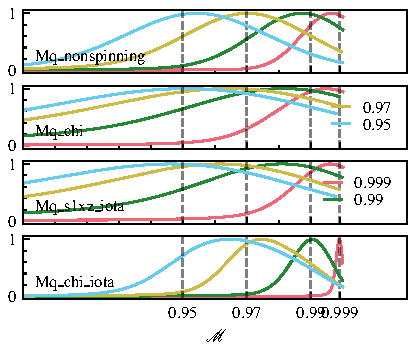
\includegraphics{metric_accuracy_hessian}
		\caption{Accuracy study with Hessian}
		\label{fig:metric_accuracy_hessian}
	\end{subfigure}\hfill
	\begin{subfigure}{0.4\textwidth}
		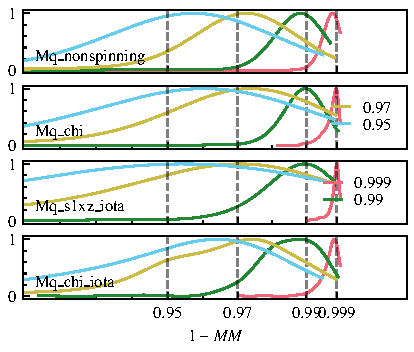
\includegraphics{metric_accuracy_parabolic}
		\caption{Accuracy study with Parabolic fit Hessian}
		\label{fig:metric_accuracy_parabolic}
	\end{subfigure}
	\caption{Metric accuracy study for different manifolds, using the two proposed metric computation methods - hessian (left) and parabolic fit hessian (right).
	Each histogram shows the distribution of matches between $15000$ pairs of random points with metric match $0.95, 0.97, 0.99, 0.999$. The masses of the test points are chosen in the $M-q$ space within the rectangle ${[20, 50] M_\odot \times [1,5]}$; the other variables are chosen in the largest possible set of accetable values.}
	\label{fig:metric_accuracy}
\end{figure*}


As the bank generation method relies on the assumption that the metric match provides a good approximation to the match, it is crucial to have a quantitative estimation of the goodness of this assumption.

To do this, we choose 4 different manifolds of templates $\mathcal{B}$ which cover different physical quantities of interests. For each manifold, we uniformly draw $15000$ samples and we compute the metric at each of this point.
For each of this points we pick a random point at a constant metric match $\mathcal{M}_{\text{metric}}$ with respect to the center $\theta_C$\footnote{
This amounts to draw a point on the constant match ellipsoid centerd in
$\theta_C$: $\{\theta \; | \; d_{\text{metric}}(\theta,\theta_C) \leq 1-\mathcal{M}_{\text{metric}} \}$.
}
For each of this point, we compute the actual match~\eqref{eq:match} and we plot the histogram of such values. For an increasingly accurate metric approximation, we should see an increasingly narrow histogram peaked around $M_{\text{metric}}$.
We repeat the experiment for $\mathcal{M}_{\text{metric}} = 0.95, 0.97, 0.99, 0.999$.

The experiment is performed on the following manifolds:
\begin{itemize}
	\item \texttt{Mq\_nonspinning} with coordinates $M = m_1+m_2, q = m_1/m_2>1$ in the rectangle $[20, 50] M_\odot \times [1,5]$
	\item \texttt{Mq\_chi} with coordinates $M, q, \chi = s_{1z} = s_{2z}$ in the rectangle $[20, 50] M_\odot \times [1,5] \times [-0.99, 0.99]$
	\item \texttt{Mq\_s1xz\_iota} with coordinates $M, q, s_{1}, \theta_1, \iota$ in the rectangle $[20, 50] M_\odot \times [1,5] \times [0, 0.99] \times [0,\pi]  \times [0,\pi]$, where $s_1, \theta_1$ are the polar coordinates of $(s_{1x}, s_{1z})$
	\item \texttt{Mq\_chi\_iota} with coordinates $M, q, \chi, \iota$ in the rectangle $[20, 50] M_\odot \times [1,5] \times [-0.99, 0.99] \times [0,\pi]$
\end{itemize}

For the first two manifolds we use the approximant \texttt{IMRPhenomD}, whereas for the latter two we use \texttt{IMRPhenomPv2} and \texttt{IMRPhenomXPHM}. The frequency range for the metric computation is always set to be $[10, 1024]Hz$.
We repeat the experiment for the two metric computation methods described in sec.~\ref{sec:metric}: {\it hessian} and {\it parabolic fit hessian}.
The results are reported in fig.~\ref{fig:metric_accuracy}.

By looking at the results for the metric hessian fig.~\ref{fig:metric_accuracy_hessian}, we note indeed a large scatter in the match values at a constant metric match. On the other hand, the random fluctuations of the match are well centered around the expected value.
For the manifold \texttt{Mq\_chi\_iota} (where an HM approximant was used), the situation is different, as the hessian metric provides a more reliable approximation to the match. However, in this case the match is underestimated by the metric match.

The picture changes drastically for the parabolic fit hessian fig.~\ref{fig:metric_accuracy_parabolic}: here the scatter of the match values is smaller (i.e. the metric approximation is more reliable) but the metric underestimates the match.

Trying to draw some general conclusions, the {\it hessian} metric approximation can yield to large errors in match estimation but it is not biased: given two points with a metric match $\mathcal{M}_{\text{metric}}$ the most likely match value between them is $\mathcal{M} = \mathcal{M}_{\text{metric}}$. 
On the other hand, the {\it parabolic fit hessian} metric approximation has smaller discrepancies but it consisently underestimates the match: if two points have metric match $\mathcal{M}_{\text{metric}}$ the most likely match value is often $\mathcal{M} > \mathcal{M}_{\text{metric}}$.
A separate conclusion holds for any HM metric. In this situation, the two metric computation methods do not differ significantly and the remarks made for the {\it parabolic fit hessian} seem to be valid.

When it comes to template placing, the overall picture is somehow conterintuitive: althogh less accurate, due to its smaller bias, the {\it hessian} metric has better performance, whereas the {\it parabolic fit hessian} leads to an overcovered bank (as it underestimates the match). This will be manifest in sec.\ref{sec:HM_bank} where an HM bank, covering the manifold \texttt{Mq\_chi\_iota}, is shown to overcover the space. The same bias is not observed in non-HM banks generated with the hessian metric.

For this reason, in the remainder of the paper we will focus only on the {\it hessian} metric, as the other alternative seem


%As discussed above, the metric approximation to the match eq.~\eqref{eq:metric_definition} is only valid in the limit of small {\it coordinate} distance $||\Delta\theta||$ and we cannot rely on the metric for larger distance. For this reason, in fig.~\ref{fig:metric_accuracy} we only consider pairs of points satisfying $||\Delta\theta||\leq 1$. We see that, under this condition, the metric provides a nice approximation to the match: the actual matches are only mildly scattered around their metric match and the random fluctuations are well centered around the expected value. The only exception to this is the manifold \texttt{Mq\_chi\_iota}, which includes Higher Order Modes (HM). In this situation, even in the limit $||\Delta\theta||\leq 1$, the metric match {\it underestimates} the actual match. The reason for this is still unknown and requires more investigation. This discrepancy is consistent with the discrepancy between match and metric match observed for the HM bank generated in sec.~\ref{sec:HM_bank}.
%As already seen, the metric approximation breaks down for $||\Delta\theta|| \geq 1$. This can be clearly seen in fig.~\ref{fig:metric_accuracy_distance}, where we plot, for each of the $15000$ pairs of points considered, the match $\mathcal{M}$ against the coordinate distance $||\Delta\theta||$. We consider only pairs of points with constant metric distance $\mathcal{M}_{\text{metric}} = 0.97$. The results are straightforward to interpret: for $||\Delta\theta|| \leq 1$ the metric approximation works well and we see that the actual matches are scattered around the value of $0.97$. On the other hand, for larger distances the true matches can be as low as $0$, even though the metric predicts a match of $0.97$.

%This happens whenever an eigenvalue of the metric is too small (i.e. the metric is close to be degenerate). In this situation, the metric will predict an unphysically large coordinate distance. There might be several ways to cure this, which will be investigated in future work:
%\begin{itemize}
%	\item Fix the metric eigenvalues by looking at the actual match \stefano{I already did this. Should we mention this somewhere?}
%	\item Insert an exponential ``damping" term $\propto e^{-||\Delta\theta||}$ to the metric distance eq.~\eqref{eq:metric_definition}. This would make the metric predictions more physical at the price of leaving the bilinear approximation to the match.
%\end{itemize}
%The tuning and the validation of those two methods will be investigated in future works.

\stefano{Uncorfotable question: why HM metric works also for $||\Delta\theta||>1$?? This challenges our understanding: we need to take into account the magnitude of the eigenvalues, but how? Just plot $||\Delta\theta||/|M|^{1/D}$? Lots of thinking there...}

\begin{figure*}[t!]
	\centering
	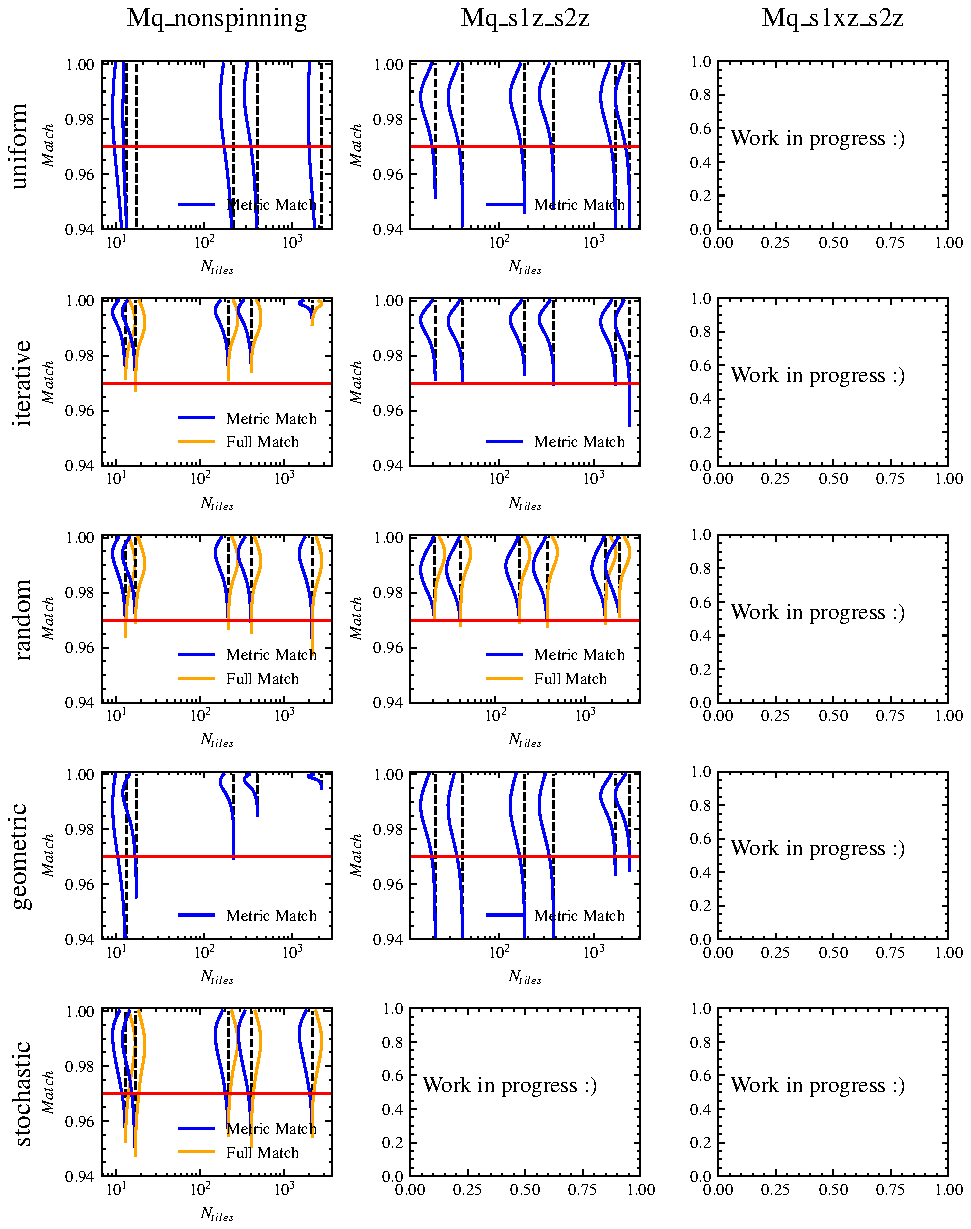
\includegraphics[width=.75\textwidth,keepaspectratio]{placing_validation}
	\caption{Results for the validation of the placing methods on $0.97$ minum match banks. Each row refers to a different placing method whereas each column refers to a different manifold being sampled. In each plot, we report with a cross the number of tiles $N_{\text{tiles}}$ against the number of templates $N_{\text{templates}}$ of the bank.
	The diamond plot refers to the fitting factor distribution of an injection study performed on the banks. The fitting factor is computed both with the match (orange) and the metric match (blue). The histograms are normalized to arbitrary units and a red tick marks the $0.97$ match threshold.
	The injections studies are performed with $5000$ injections for \texttt{Mq\_s1xz} and $1000$ injections in the remaining cases.
	}
	\label{fig:placing_validation}
\end{figure*}

\subsection{Placing methods accuracy} \label{sec:placing_accuracy}

\stefano{should we write somewhere the manifold naming convention? or do we rather describe it as it is whenever necessary?}

Here we compare the performances of different placing methods: \textit{uniform}, \textit{random} and \textit{stochastic}.
This will be helpful to understand their ranges of applicability and possibile limitations in their use.

We consider 3 different manifolds:
\begin{itemize}
	\item \texttt{Mq\_nonspinning} with coordinates $M, q$ in the rectangle $[30, 50] M_\odot \times [1,5]$
	\item \texttt{Mq\_chi} with coordinates $M, q, \chi $ in the rectangle $[30, 50] M_\odot \times [1,5] \times [-0.99, 0.99]$
	\item \texttt{Mq\_s1xz} with coordinates $M, q, s_{1}, \theta_1$ in the rectangle $[40, 50] M_\odot \times [1,5] \times [0, 0.99] \times [0,\pi]$
\end{itemize}
For the first two manifold we use the approximant \texttt{IMRPhenomD}, while for the latter we use \texttt{IMRPhenomPv2}.
For each manifold, we generate different tilings with a different number of tiles and we generate a bank with $0.97$ minimum match.
To compute the metric, we use the PSD for Handford measured on the first three months of O3, as publicly released by the LVK collaboration \cite{https://dcc.ligo.org/LIGO-T2000012/public}.

We then perform an injection study on the banks thus generated and we report the histogram of the fitting factor for both the match and the metric match. We choose $1000$ injections for the first two manifold and $5000$ injections in the latter\footnote{
The number of injections are the same order of magnitude of the number of templates in the bank, hence we expect the results obtained to be robust.}.
For the stochastic placement we set the parameter $N_{max} = 100$, while for the random method we employ $1000 N_{\text{templates}}$ livepoints (where $N_{\text{templates}}$ is defined in eq.~\eqref{eq:N_templates}).
The results are shown in fig.~\ref{fig:placing_validation}.

By looking at the number of templates placed by the {\it uniform} method, we see that they all grow with the number of tiles until a certain upper limit. This is the expect behavior of a good tiling generation method. Indeed we expect that an incresing number of tiles provides a better estimation of the overall volume of the space until the estimation converges to the actual value in the limit of infinite tiles. Moreover, according to eq.~\eqref{eq:N_templates}, the number of templates placed by the uniform method is essentially a measure of volume.
The fact that the tiling generation method is able to reach a stable estimation of the number is then a confirmation of its robustness in estimating the actual volume of the space.

We now analyse the properties of the different methods.

We note that the {\it uniform} placing method understimates the number of templates with respect to the other two methods. Moreover, it provides a poor coverage of the space, since a very large fraction of the injections has a fitting factor below the target $0.97$. This is expected since, unlike other methods, all the templates are drawn independently from each other: this causes great oscillation in the templates densities, generating overdense and underdense regions.
However, it is important to note that, as mentioned before, this methods can still be useful to provide a quick estimation of the bank features and in practice it can be used in the exploratory analysis preceding the generation of a bank.

The {\it random} method provides very nice coverage properties of the two non-precessing manifolds (\texttt{Mq\_nonspinning} and \texttt{Mq\_chi}): this can be seen by the excellent fitting factor of the injection performed. Moreover, the method performances do not depend on the number of tiles.
For the precessing manifold, \texttt{Mq\_s1xz}, the method's performances sligthly deteriorates as can be seen by the large tails in the fitting factor histogram.
This is a well known feature of this placing method that leads to bad coverage whenever the metric changes drastically across the space. In this situation, a livepoint from a tile with a low $\sqrt{|M|}$ can ``kill" other livepoints in an unphysically large portion of the parameter space (see the discussion in sec.~\ref{sec:metric_accuracy}). For this reason, the high density regions ca be underpopulated due to the breaking down of the metric approximation. A possible solution for this is to introduce a cut-off on the effect of the metric, hence limiting the unphysical long range action of a quasi-degenerate metric: this will be the scope of future work.
Despite this pathology, the {\it random} method still remains a valid option due to its robustness and speed.

As shown by our results, the {\it stochastic} method is always able to cover the space with the appropriate minimum match. This very nice performance is of course expected: this placing method (with some variations) is the state of the art of bank generation and has proven to be reliable.
On our implementation of the method, we note that (especially for \texttt{Mq\_chi}) the number of templates {\it do} depend on the number of tiles: this can lead to overcover the space. The reason for that lies in the stopping condition implemented. We stop proposing new templates inside a tile after $N_{max}$ iterations without a template being added in that tile. Hence of course, a large number of tiles provides a more stringent terminating condition (at a constant $N_{max}$) than a small number of tiles.
A possible solution for this would be to impose a stopping condition on the global volume: this however would consume a lot of computational power as it does not provide a mechanism to stop making proposals in tiles that are already ``full".
A way around this shortcoming is to tune $N_{max}$ so as to achieve the desidered performance: this can be quickly checked by computing the metric fitting factor on an injection set.

\stefano{Are they clear from the text?}
Take home messages:
\begin{itemize}
	\item Uniform: gets the order of magnitude but does not do a good job in placing templates
	\item Random: Perfect as long the tiles have similar metric: otherwise weird problems
	\item Stochastic: perfect but it may depend on the number of tiles
\end{itemize}


\begin{table*}[t!]
	%\centering
	\setlength\extrarowheight{1pt}
	 \begin{tabular}{l l c c c c} 
	 \hline
	 	%header
	 \multicolumn{1}{c}{\phantom{Bank name}} & \multicolumn{1}{c}{\textbf{Ranges}} & 
	 \multicolumn{2}{c}{
		\begin{tabular}{c c} \multicolumn{2}{c}{\textbf{Size}}  \\ \texttt{sbank} & \mbank \\ \end{tabular}	 
	 } &
	  \multicolumn{2}{c}{
		\begin{tabular}{c c} \multicolumn{2}{c}{\textbf{Time}}  \\ \texttt{sbank} & \mbank \\ \end{tabular}	 
	 }\\	 
	 %\multicolumn{1}{c}{\phantom{Bank name}} & \multicolumn{1}{c}{\textbf{Ranges}} & \multicolumn{2}{c}{\textbf{Size}} \\	 
	 %\multicolumn{1}{c}{\phantom{Bank name}} & \multicolumn{1}{c}{\phantom{Ranges}} & \multicolumn{1}{c}{\texttt{sbank}} & \multicolumn{1}{c}{\mbank} \\
	 \hline
	 Nonspinning & \begin{tabular}{@{}l@{}} $M\in [30,50] M_\odot$ \\ $q\in [1,5]$   \\ \end{tabular}  &
	 		396 & 442 & $O(\text{hours})$ & $O(\text{seconds})$ \\
	 \cdashline{1-6}
	 Aligned spin & \begin{tabular}{@{}l@{}} $M\in [30,50]$ \\ $q\in [1,5]$ \\ $s_{1z}, s_{2z}\in [-0.99,0.99]$  \\ \end{tabular}  &
	 	3275 & 4108 & $O(\text{days})$ & $O(\text{minutes})$ \\
	 \cdashline{1-6}
	 Aligned spin low mass & \begin{tabular}{@{}l@{}} $M\in [10,30]$ \\ $q\in [1,5]$ \\ $s_{1z}, s_{2z}\in [-0.99,0.99]$  \\ \end{tabular}  &
	 	48000 & 127178 & $O(\text{weeks})$ &  $O(\text{hours})$\\
%	 \cdashline{1-4}
%	 GstLAL O3 bank & \begin{tabular}{@{}l@{}} $M\in [33,100]$ \\ $q\in [1,10]$ \\ $s_{1z}, s_{2z}\in [-0.99,0.99]$  \\ \end{tabular}  &
%	 	60166 & 15549 \\
	 \hline
	 \end{tabular}
	 \caption{Comparison between the performance of \mbank and  \texttt{sbank} on 3 chosen regions of the parameter space.
	 For each bank, we report the range of parameters covered by the templates, the size of the banks generated by the two methods as well as the order of magnitude of the generation time. The frequency range for all the banks is set to be $f\in [15,1024] Hz$.
	 The details of the injection studies are shown in figure~\ref{fig:sbank_comparison}.
	 }
 	 \label{tab:sbank_comparison}
\end{table*}


\subsection{Comparison with \texttt{sbank} }\label{sec:sbank_comparison}

\stefano{Should I make an mbank bank also for the parabolic hessian? Might be interesting for validation...}
\texttt{sbank} \cite{sbank} is the standard tool used by the LIGO-Virgo collaboration to generate large template banks for analysis and as such, it has been used sucessfully in the past three observing runs by several pipelines.
For this reason, it is very important to compare the performance of our code against the benchmark set by \texttt{bank}. The comparison is based on the size, speed and effectualness of the banks generated.

We generate three non-precessing template banks with both codes:
\begin{itemize}
	\item A {\it non spinning} bank
	\item An {\it aligned spins} bank
	\item An {\it aligned spins low mass} bank
\end{itemize}
The ranges of the parameter space covered by the three banks are reported in table~\ref{tab:sbank_comparison}. All the banks cover the frequency range $f\in [15,1024] Hz$ and are generated using the PSD measured during O2 between GPS times $1164556817$ and $1187740818$.
In the same table, we report the size of the banks generated and their generation time. In fig.~\ref{fig:sbank_comparison}, we report the result of an injection study on the three pair of banks.

The first striking feature we observe is that \mbank has a consistently higher number of templates. For the first two banks it has around 30\% more templates whereas in the last case it has around 100\% more templates. This means that the metric template placement tends to overcover the space. This is a kown feature (also observed in \cite{}) and it is inherent to the method: it is the price to pay for a huge speed up.

Looking at the injections fitting factor histograms in fig.~\ref{fig:sbank_comparison}, we see that the histograms have similar tails. This means that \mbank is able to cover the space leaving as few underdense regions as \texttt{sbank}. On the other hand, we see the peak in the fitting factor distributions for \mbank is systematically higher that the one by \texttt{sbank}. This is consistent with the fact that \mbank has more templates, which must provide a higher average fitting factor.

When considering the generation times, we see that \mbank is {\it orders of magnitude} faster than \texttt{sbank}. This huge speed up is precisely what makes \mbank convenient, especially to cover very large volumes: it may overcover the space but it provides a substantial speed-up, making feasible the covering of new regions of the parameter space.

\begin{figure}[t]
	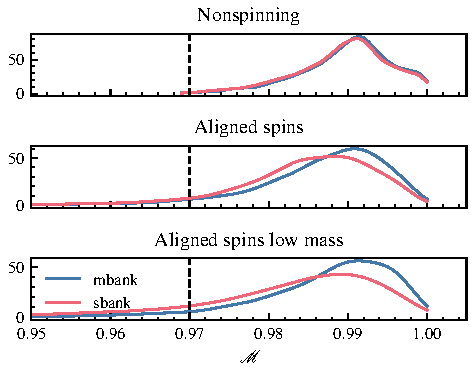
\includegraphics{sbank_comparison}
	\caption{Histogram for the fitting factors of the banks used to compare \mbank and \texttt{sbank}. For each parameter space considered, we randomly draw $5000$ points (injections) from the tiling used to generate the \mbank bank and we compute the fitting factor of these injections against the two banks. We report the distribution of fitting factor in the histograms. For visualization purposes, we plot the $0.97$ line, which corresponds to the minimum match of the banks.
	The details of the banks generated are reported in table~\ref{tab:sbank_comparison}.
	}
	\label{fig:sbank_comparison}
\end{figure}

%%%%%%%%%%%%%%%%%%%%%%%%%%%%%%%%%%%%%%%%%%%%%%%%%%%%%%%

	%%%%%%%%%%%%%%%%%%%%%%%%%%%%%%%%%
\section{Bank generation: three case studies} \label{sec:bank_generation}

To demostrate the capabilities of our method, we use \mbank to generate three large banks covering interesting un-explored regions of the parameter space.
They are:
	\begin{itemize}
		\item A precessing bank
		\item An Intermediate Mass BH bank with Higher Order Modes
		\item A nonspinning eccentric bank
	\end{itemize}
Generating these banks with a standard approach is extremely costly and such cases represent the ideal situation where \mbank is most useful.

For each bank, we perform an injection study, as described in sec.~\ref{sec:sbank_comparison}. We generate $40000$ inections randomly drawn from the tiling: the results are reported in fig.~\ref{fig:bank_injections}. We also plot the templates of the banks in fig.~\ref{fig:bank_scatter}.
In table~\ref{tab:casestudy_banks}, we summarize the features of each bank, such as the size and the range of physical quantities that they cover.
All the banks are generated with a minimum match $MM$ requirement of $0.97$, using the {\it stochastic} placement method.
As above, we use the Hanford detector PSD measured during O3, as publicly released by the LVK collaboration \cite{https://dcc.ligo.org/LIGO-T2000012/public}.

In the following subsections, we will describe in details the generated banks and comment on their usability and accuracy.

\subsection{A precessing bank}\label{sec:precessing_bank}
	
In this high mass {\it precessing} bank, we assign a two dimensional precessing spin to the most massive BH. We then consider only the x and z components of the spin $s_1$ and we sample in polar coordinates. The masses are sampled in the space (total mass - mass ratio) $M,q$.  Thus the metric is evaluated at the coordinates point $\theta = (M, q, s_1, \theta_1)$. In table~\ref{tab:sbank_comparison}, we report the ranges covered by each of this quantities. We use the approximant \texttt{IMRPhenomPv2}.

This choice of variable is based on the fact that the effect of precession can be absorbed in a single {\it effective spin parameter}, assigned to the most massive BH of a binary \cite{}. Thus this physical approximation allows us to cover a large number or precessing signal using a (relatively) small number of variables. \stefano{This argument works better if we consider also s2z. Shall we do this?}

By looking at the scatter plots of the templates, it is manifest the effect due to the discretization error introduced by the tiles: this causes a discontinuity in the template density. Of course, this effect is unphysical and would have been avoided by a purely stochastic placing method.
Another possible source of discontinuity can be traced back to numerical noise in the numerical gradients of the waveforms. Depending on the approximant, the gradients (hence the metric) may not behave smoothly all across the parameter space, thus explaining (partly) the hard discontinuities.

Nevertheless, the injection recovery (fig.~\ref{fig:bank_injections}) is satysfying with only $3.45\%$ of the $40000$ injections performed having a recovery less than the target match $MM = 0.97$.

By looking at fig.~\ref{fig:bank_injections}, we also note that the injection recovery computed with the metric match tends to overestimate the true injection match. The discrepancy however is small enough that the bank performance remains acceptable.

\subsection{An IMBH HM bank}\label{sec:HM_bank}

We generate a bank that includes Higher Order Modes \cite{something_about_HM} (HM). The HMs provide a more physical accurate approximation of the signal. They are more important in the strong gravity regime, thus they affect mostly the late inspiral and the merger part of the waveform.
For this reason, it is interesting to search HM data in the Intermediate Mass Black Hole (IMBH) region, characterized by a total mass $M>50 M_\odot$. An IMBH signal spends only a small time ($O(ms)$) in the detector's frequency band and thus having an accurate HM template is crucial for better detection.
We include in the bank the variables $\log M, q, \chi, \iota$, where $\chi=s_{1z}=s_{s2z}$ is the effective spin parameter and $\iota$ is the inclination angle.
As before in table~\ref{tab:sbank_comparison}, we report the ranges for each of this quantities. We use the modern HM approximant \texttt{IMRPhenomXPHM}.

The inclusion of HM makes the bank much larger (i.e. $|M|$ is larger): for reference, a non HM bank, covering the masses and $\chi$ ranges (of course, without $\iota$) has $\sim 1000$ templates: that is a 2 orders of magnitude difference!
%By looking at the scatter plot fig.~\ref{fig:bank_scatter}, we can note the effect of the discretization introduced by the tiling.

By looking at the injection recovery fig.~\ref{fig:bank_injections} it is striking the discrepancy between the recovery factor computed by the metric and the un-approximated one. Indeed, in the HM case the metric strongly {\it underestimates} the match, yielding an overpopulated bank. With the metric injection recovery, approximately $6\%$ of the injections have a recovery below $0.97$: this is consistent with the placing method used, which only ``knows" about metric matches. On the other hand, only $0.5\%$ are below the $0.98$ recovery factor: the bank generated is effectively a $98\%$ bank.
\stefano{What's the cause of the discrepancy?}
\stefano{To quantify this, should we do another plot in fig.~\ref{fig:metric_accuracy} for the XPHM approximant?}


\subsection{An eccentric nonspinning bank}\label{sec:eccentric_bank}

Finally, we generate an eccentric bank. Usually the BBH searches have focused on circular orbits.
This is well theoretically motivated, as by the time of merger, any initial orbital eccentricty will be radiated away. Nevertheless is interesting to search such signals as their detection will provide invaluable information on the BBH dynamics and the BBH formation channels and stellar evolution.
The eccentricity leaves a characteristic signature on the inspiral, thus it will be more detectable on long signals. For this reason, we focus on the {\it low} mass region $M\in [10,75] M_\odot$, where the inspiral is detectable for a longer time.
We use the approximant \texttt{EccentricFD} and we limit ourselfs to low eccentricities $e<0.3$, where the WF modelling is more realiable. Althought the choen approximant is not very accurate, we still expect it to include enough physics to provide an approximate coverage of the space.

As in the case of the HM bank, including eccentricity yields a bank orders of magnitude larger than a standard non-eccentric bank.
By looking at the injection recovery, we note that only $0.15\%$ of the injections have match below $0.97$ against the bank. Although the metric match still underestimates the fitting factor, this issue is less severe than in the HM case.

From the scatterplot fig.~\ref{fig:bank_scatter}, we note that the discontinuities introduced by the metric are less visibile. This is due to the smaller dimension of the space (3 against 4 of the previous cases), which makes easier to cover the space with a reliable tiling. Moreover, since the approximant \texttt{EccentricFD} is analytic, the metric has a smoother dependence on the parameter space, which may also help to avoid discontinuities in template density.


\begin{table*}[t!]
	\centering
	\setlength\extrarowheight{1pt}
	 \begin{tabular}{l l l c c} 
	 \hline
	 %\multicolumn{1}{c}{\phantom{Name}} & \multicolumn{1}{c}{\textbf{Ranges}} & \multicolumn{1}{c}{\textbf{Setting}} & \multicolumn{1}{c}{\textbf{Size}} \\
	 \multicolumn{1}{c}{\phantom{Bank name}} & \multicolumn{1}{c}{\textbf{Ranges}} & \multicolumn{1}{c}{\textbf{Settings}} &  
	 \multicolumn{2}{c}{
		\begin{tabular}{c c} \multicolumn{2}{c}{\textbf{Size}}  \\ $N_{\text{templates}}$ & $N_{\text{tiles}}$ \\ \end{tabular}	 
	 } \\
	 \hline
	 Precessing & \begin{tabular}{@{}l@{}} $M\in [25,100] M_\odot$ \\ $q\in [1,5]$  \\ $s_1\in [0,0.99]$ \\$\theta_1\in [0, \pi]$ \\ $f\in [15,1024] Hz$ \\ \end{tabular}  &
	 \begin{tabular}{@{}l@{}} IMRPhenomPv2 \\ $\epsilon = 0.1$ \\ \texttt{max-depth}: 10 \\ \end{tabular}  &
	 54750 & 33774 \\
	 \cdashline{1-5}
	 IMBH HM & \begin{tabular}{@{}l@{}} $M\in [50, 600] M_\odot$ \\ $q\in [1,5]$  \\ $\chi \in [0,0.99]$ \\ $f\in [10,1024] Hz$ \\ \end{tabular}  &
	 	 \begin{tabular}{@{}l@{}} IMRPhenomXPHM \\ $\epsilon = 0.2 $ \\ \texttt{max-depth}: 8 \\ \end{tabular}  &
	 	273650 & 33792 \\
	 \cdashline{1-5}
	 Nonspinning eccentric & \begin{tabular}{@{}l@{}} $M\in [10,75] M_\odot$ \\ $q\in [1,5]$ \\ $e \in [0,0.3]$ \\ $f\in [15,1024] Hz$ \\ \end{tabular}  &
	 	 \begin{tabular}{@{}l@{}} EccentricFD \\ $\epsilon = 0.1$ \\ \texttt{max-depth}: 9 \\  \end{tabular}  &
	 	154472 & 4238 \\
	 \hline
	 \end{tabular}
	 \caption{Summary of three case study banks generate with \mbank. For each bank generated, we report the variables being sampled and their ranges. We also report the approximant and the hyperparameters $\epsilon$ and \texttt{mx-depth} used for the tiling generation as well as the bank size $N_{\text{templates}}$  and the number of tiles $N_{\text{tiles}}$. An injection study is performed in fig.~\ref{fig:bank_injections}. The templates distribution of the three banks is reported in fig.~\ref{fig:bank_scatter}.}
 	 \label{tab:casestudy_banks}
\end{table*}


\begin{figure}[t]
	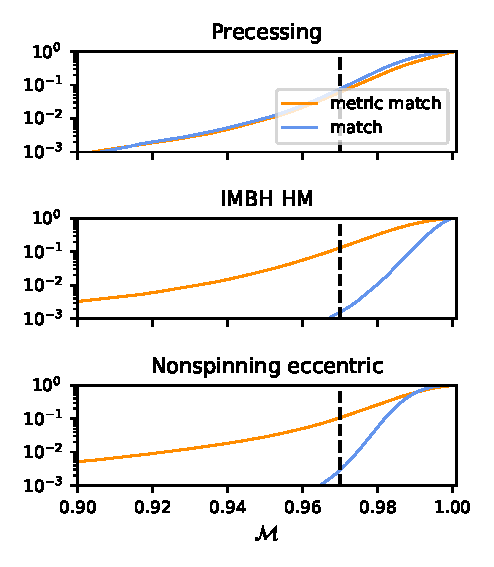
\includegraphics{bank_injections}
	\caption{
	Histogram for the fitting factors of the three case study banks. For each bank, we randomly draw $40000$ points (injections) from the tiling and we compute the fitting factor of these injections against the two banks. We report the distribution of fitting factor in the histograms both for the match and the metric match. For visualization purposes, we plot the $0.97$ line, which corresponds to the minimum match of the banks.
	The details of the banks generated are reported in table~\ref{tab:casestudy_banks}.
	}
	\label{fig:bank_injections}
\end{figure}


\begin{figure*}[t]
	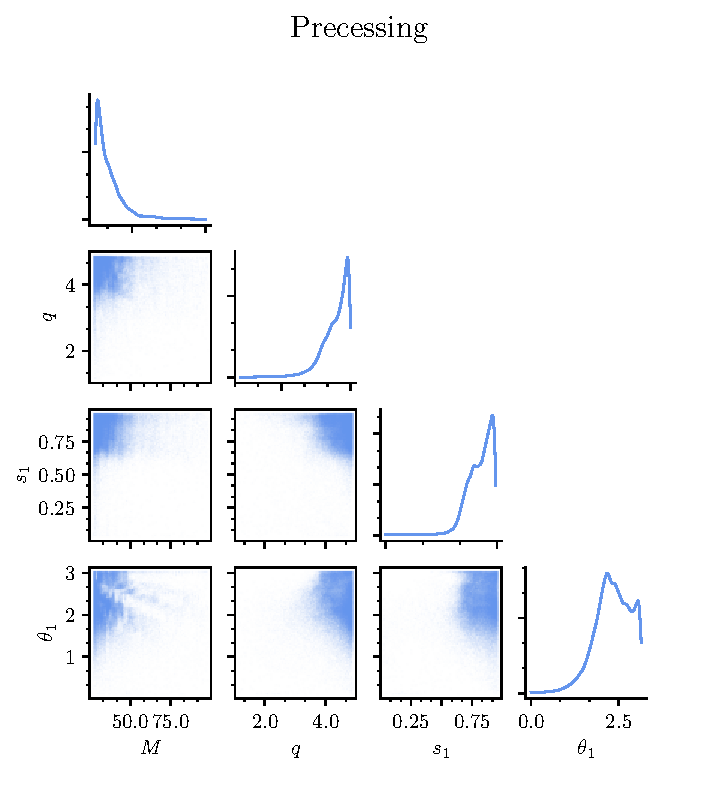
\includegraphics{bank_scatter_Precessing}\hfill
	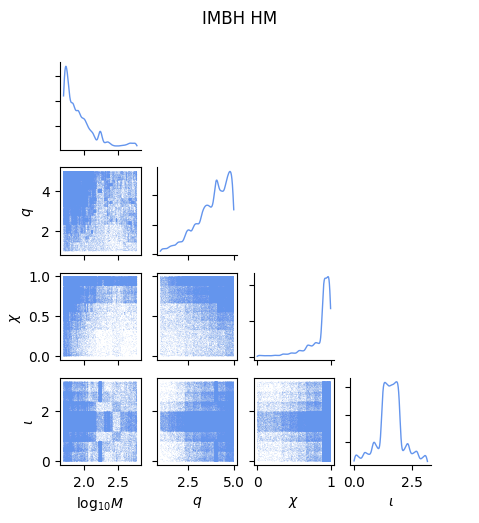
\includegraphics{bank_scatter_IMBH_HM}\hfill
	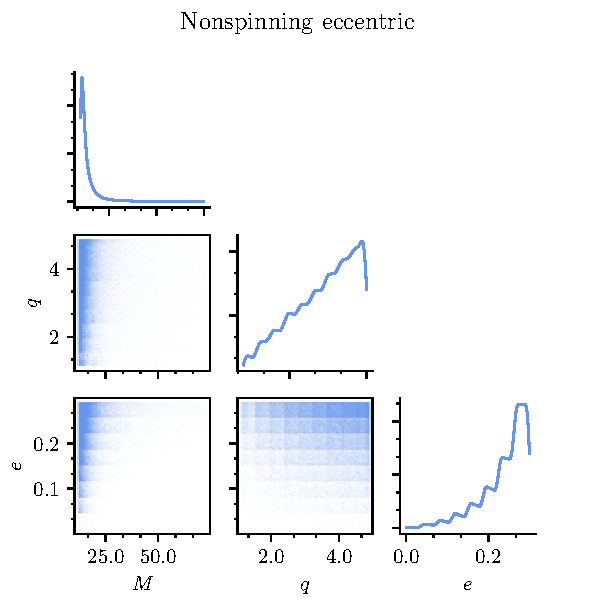
\includegraphics{bank_scatter_Nonspinning_eccentric}
	\caption{Corner plots showing the templates for the three banks described in table~\ref{tab:casestudy_banks}. }
	\label{fig:bank_scatter}
\end{figure*}

\section{Final remarks and future prospects} \label{sec:conclusion}
Usual stuff
\blindtext
\blindtext
\blindtext
\blindtext
\blindtext
\blindtext
\blindtext

	%%%%%%%%%%%%%%%%%%%%%%%%%%%%%%%%% ACKNOWLEDGMENTS
        \begin{acknowledgments}
         
          WRITEME...
        \end{acknowledgments}

	%%%%%%%%%%%%%%%%%%%%%%%%%%%%%%%%% APPENDIX
\appendix
\section{Details of the metric computation}\label{app:metric}

In this appendix we report the details of the derivation of the expression~\eqref{eq:metric_expression}, as well as the computation of the Hessian $H$ of the overlap eq.~\eqref{eq:overlap} in terms of the gradients of the waveform $h(\theta)$. 

We begin by expanding the quantity $\mathcal{M}(\theta,\theta +\Delta\theta)$ for $\Delta\theta$ around $0$. Since the $\mathcal{M}(\theta,\theta +\Delta\theta)$ has a maximum for $\Delta\theta = 0$, the leading term is quadratic in $\Delta\theta$.
We obtain:
\begin{align} \label{eq:metric_derivation}
	&\mathcal{M}(\theta,\theta +\Delta\theta) = \max_{\Delta t} \mathcal{O}(\theta, \theta + \Delta\theta, \Delta t) \nonumber\\
	& =	\max_{\Delta t} \left\{ 1+ \frac{1}{2}\left[ \partial_{ij}\mathcal{O} \Delta\theta_i \Delta\theta_j + 2  \partial_{it}\mathcal{O} \Delta\theta_i \Delta t + \partial_{tt}\mathcal{O} (\Delta t)^2 \right] \right\}  \nonumber \\
	&= 1 + \frac{1}{2}\left[ \partial_{ij}\mathcal{O} - \frac{\partial_{it}\mathcal{O} \partial_{jt}\mathcal{O}}{\partial_{tt}\mathcal{O}}\right] \Delta\theta_i \Delta\theta_j
\end{align}
where all the derivatives are evaluated at ${\Delta\theta = \Delta t = 0}$ and the explicit time maximization yields
${\Delta t = -\frac{\partial_{it}\mathcal{O} \Delta\theta_i}{\partial_{tt}\mathcal{O}}}$.

From the above eq.~\eqref{eq:metric_derivation}, we can read the expression for the metric in eq.~\eqref{eq:metric_expression} recognizing in the derivatives $\partial\partial\mathcal{O}|_{\Delta\theta, \Delta t = 0}$ the components of the Hessian matrix $H$ of the overlap.

We now compute the Hessian of the overlap as a function of the gradients of the {\it normalized} waveforms.
We have\footnote{
A constant factor in front of the frequency in the fourier transform does not affect the result. For this reason, we dropped the constant $2\pi$ in the exponential.}:
\begin{align}
	\partial_i \mathcal{O} &= \frac{1}{\mathcal{O}} \left[ \rescalar{\hat{h}}{\hat{h}e^{ift}}\rescalar{\hat{h}}{\partial_i\hat{h}e^{ift}} + \imscalar{\hat{h}}{\hat{h}e^{ift}}\imscalar{\hat{h}}{\partial_i\hat{h}e^{ift}} \right]\\
	\partial_t \mathcal{O} &= \frac{1}{\mathcal{O}} \left[ \rescalar{\hat{h}}{\hat{h}e^{ift}}\rescalar{\hat{h}}{\hat{h}if e^{ift}} + \imscalar{\hat{h}}{\hat{h}e^{ift}}\imscalar{\hat{h}}{\hat{h}if e^{ift}} \right]
\end{align}
Differentiating another time, after some rearrengments, we get:
\begin{align}
H_{tt} &= \frac{\partial^2 \mathcal{O}}{\partial t \partial t } \left|_{\Delta\theta, t = 0} \right.
								= \rescalar{\hat{h}}{\hat{h}f}^2 - \rescalar{\hat{h}}{\hat{h}f^2} \label{eq:H_tt}\\
H_{ti} &= \frac{\partial^2 \mathcal{O}}{\partial \Delta \theta_i \partial t } \left|_{\Delta\theta, t = 0} \right.
								= - \imscalar{\hat{h}}{\partial_i \hat{h}f} + \imscalar{\hat{h}}{\partial_i\hat{h}} \rescalar{\hat{h}}{\hat{h}f} \label{eq:H_ti}\\
H_{ij} &= \frac{\partial^2 \mathcal{O}}{\partial \Delta \theta_i \partial \Delta \theta_j }\left|_{\Delta\theta, t = 0} \right.
								= \rescalar{\hat{h}}{\partial_i\partial_j\hat{h}} +\imscalar{\hat{h}}{\partial_i\hat{h}} \imscalar{\hat{h}}{\partial_j\hat{h}} \label{eq:H_ij}
\end{align}

To move further, we express the normalized waveform derivatives in terms of the non normalized ones. We get:
\begin{align*}
	\bullet&\quad \partial_i \scalar{h}{h} = \scalar{\partial_i h}{h}+ \scalar{h}{\partial_i h} = 2 \rescalar{h}{\partial_i h} \\
	\bullet&\quad \partial_i \hat{h} =\frac{1}{\rescalar{h}{h}^{3/2}} \left[ \rescalar{h}{h}\partial_i h -  \rescalar{h}{\partial_i h} h \right]	\\
	\bullet &\quad \partial_i \partial_j \hat{h} = \frac{1}{\rescalar{h}{h}^{1/2}} \partial_{ij}h 	+3 \frac{1}{\rescalar{h}{h}^{5/2}} \rescalar{h}{\partial_i h}\rescalar{h}{\partial_j h}h \\
	&- \frac{1}{\rescalar{h}{h}^{3/2}} \left[\rescalar{h}{ \partial_{ij} h} h + \rescalar{\partial_i h}{\partial_j h}  h
		+2\rescalar{h}{\partial_{(i} h} \partial_{j)} h \right]
\end{align*}
where $A_{(ij)} = \frac{1}{2}(A_{ij}+A_{ji})$ denotes symmetrization.

Plugging this into the equations~\eqref{eq:H_tt}-\eqref{eq:H_ij}, we get:
\begin{align}
	H_{tt} &= \frac{1}{\rescalar{h}{h}^{2}} \rescalar{{h}}{{h}f}^2 - \frac{1}{\rescalar{h}{h}} \imscalar{h}{{h} f^2 } \label{eq:H_tt_grad} \\
	H_{ti} &= \frac{1}{\rescalar{h}{h}^{2}} \Big\{ \imscalar{h}{\partial_i {h}} \rescalar{{h}}{{h}f} +\rescalar{h}{\partial_i {h}} \imscalar{h}{hf} \Big\} \nonumber \\
	&- \frac{1}{\rescalar{h}{h}} \imscalar{h}{\partial_i{h} f } \label{eq:H_ti_grad} \\
	H_{ij} &=  \frac{1}{\rescalar{h}{h}^{2}} \Big\{ \rescalar{h}{\partial_i {h}} \rescalar{{h}}{\partial_j {h}} +\imscalar{h}{\partial_i {h}} \imscalar{h}{\partial_j {h}} \Big\} \nonumber \\
	&- \frac{1}{\rescalar{h}{h}} \rescalar{\partial_i h}{\partial_j {h}} \label{eq:H_ij_grad} 
\end{align}

Such expressions, togheter with eq.~\eqref{eq:metric_expression} fully specify the metric computation.
The gradients $\partial_i h$ of the waveform can be computed with an accurate finite difference scheme.

	%%%%%%%%%%%%%%%%%%%%%%%%%%%%%%%%% BIBLIOGRAPHY
	\bibliography{biblio.bib}
	\bibliographystyle{ieeetr}

\end{document}



